\documentclass[a4paper,18pt]{article}
% needs to be compiled with xelatex
\usepackage{eso-pic,graphicx}
\usepackage{lipsum}
\usepackage{background}
\usepackage{fontspec}
%\usepackage[top=2cm, bottom=2cm, outer=0cm, inner=0cm]{geometry}
\usepackage[pass,a4paper]{geometry}

\setmainfont{Didact Gothic}
\linespread{1.4} % 1.6 is double
\backgroundsetup{
scale=1,
angle=0,
opacity=1,  %% adjust
contents={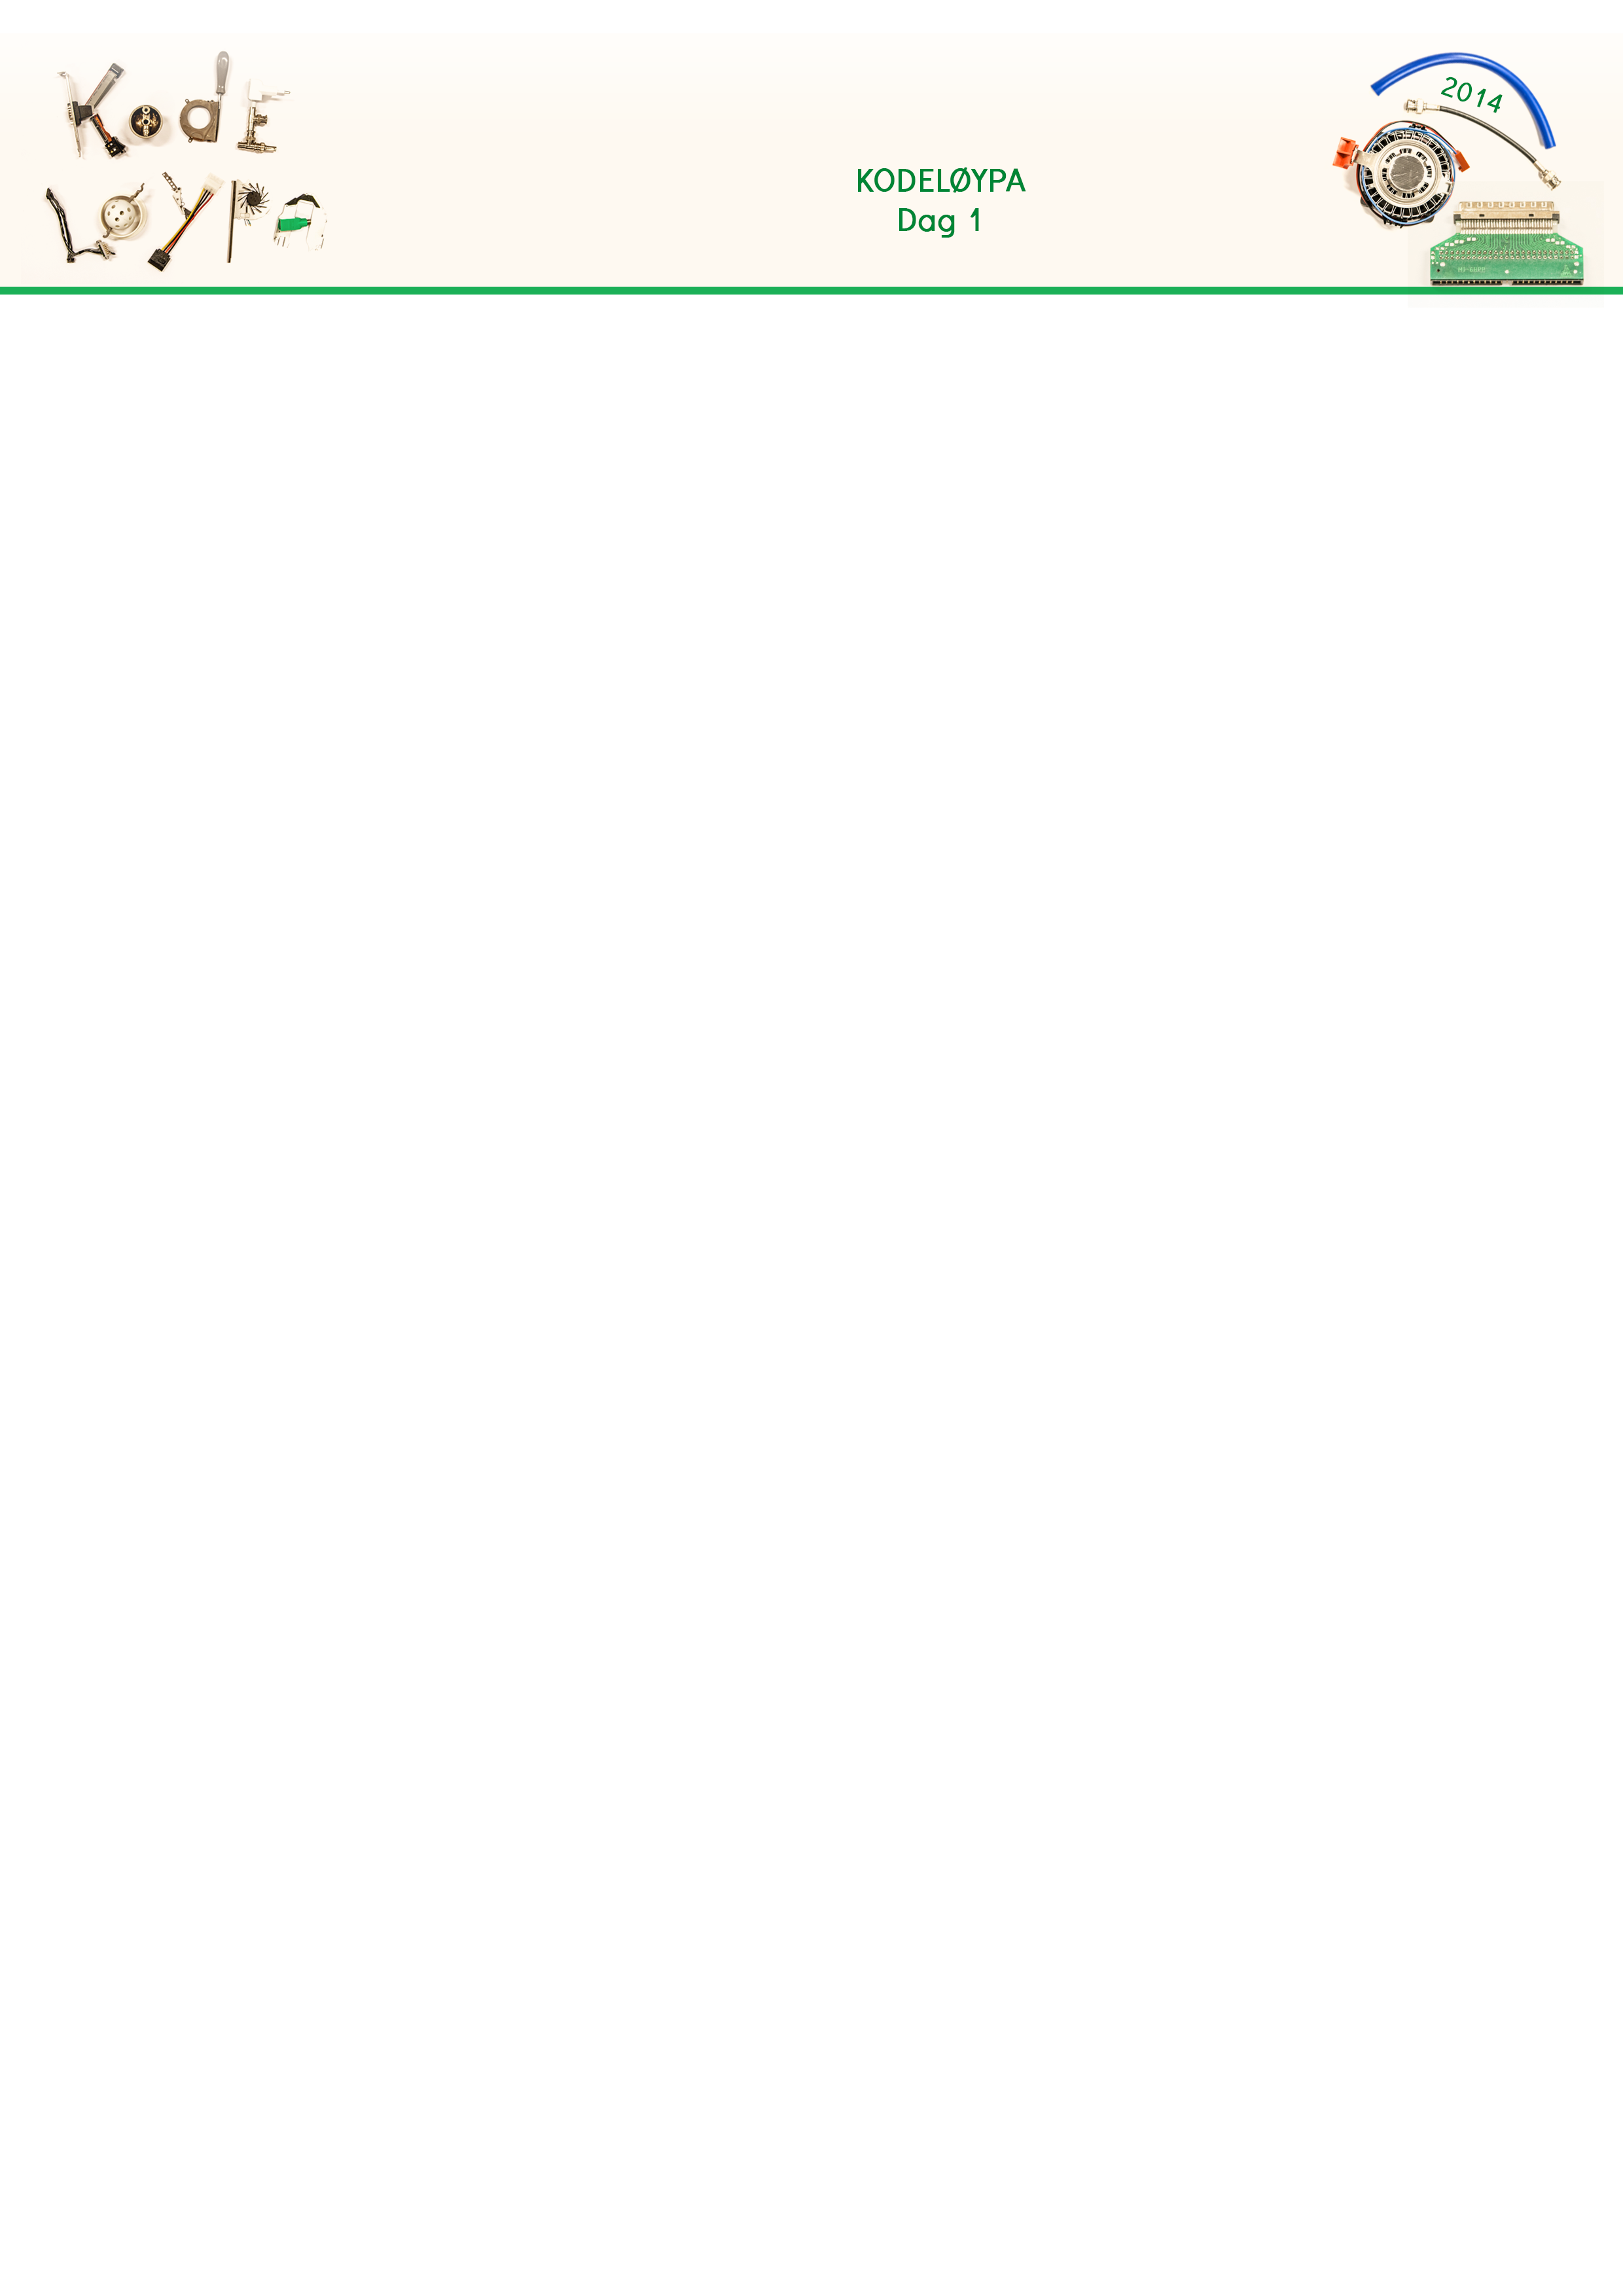
\includegraphics[width=\paperwidth,height=\paperheight]{background}}
}
\setlength{\parskip}{13pt}
\setlength\parindent{0pt}

\newcommand{\block}[2][-0.4]{\raisebox{#1\height}{\includegraphics{#2}}}
%$\vcenter{\hbox{
\includegraphics{move} }}$

\begin{document}
\begin{large}
%Vi bruker \block{move} for å flytte på 2. Også bruker vi en \block[-0.32]{flag}.
Programmet vi skal bruke den første dagen er Scratch. I Scratch er det mulig å lage animasjoner ved å gi 
kommandoer til figurene. Disse kommandoene ser ut som blokker i Scratch. Den første blokken vi skal 
bruke er \block{move}. Dra den over til kodeområdet. Dobbeltklikk på den for å se hva den gjør.

Det er mulig å sette sammen flere blokker for å få en gruppe med kommandoer.
Bytt til \block{looks} og dra over \block{say_hello} slik at den fester seg under move-blokken. Dobbeltklikk 
på blokkgruppen for å se om det fungerer som forventet.

Oppgaver
\\
\textit{Ikke vær redd for å prøve ut ting! Det er lov å finne ut av hva andre blokker gjør. Hvis dere ikke
får hjelp med en gang, skriv ned det dere lurer på og gå videre til neste oppgave eller side.
Noen ganger står det dere lurer på på neste side.}
\begin{itemize}
    \item Få katten til å gå frem, si noe og gå bakover.
    \item Endre fargen til katten hver gang den beveger seg.
        \begin{itemize}
            \item Hint: se om det er en blokk i \block{looks} som gjør fargeendringer.
        \end{itemize}
\end{itemize}

\newpage

Etterhvert som dere prøver dere frem, kan det bli ganske rotete i kodeområdet. Dere kan dra blokker eller 
blokkgrupper tilbake til området til venstre for å slette dem. Hvis dere står fast er det ofte lurt å 
fjerne noen blokker. Det gjør det lettere å se hva som skjer. 

Noen ganger fungerer det ikke fordi Scratch gjør alt så fort at dere ikke ser endringen. I slike tilfeller
er det lurt å bruke \block{wait}, som finnes i \block{control}.

Alle piksler i animasjonsområdet har en posisjon i koordinater i Scratch. Posisjon 0,0 er i midten av 
animasjonsområdet. \block{go_to} er nyttig på starten av kode som flytter på figurer. Da slipper dere å dra figurer 
tilbake hver gang dere vil teste animasjonen.

For å tilbakestille effekter og størrelsen til figuren, bruk \block{clear_graphics}
og \block{reset_size}, som begge ligger i \block{looks}.

\newpage

Det er mulig å kontrollere når noe skjer i Scratch. Det vil si, når dere klikker et sted eller trykker en tast, 
starter utføring en blokkgruppe. For å gjøre det, trenger blokkgruppen å starte med en av blokkene som Scratch 
kaller «hattblokker». Disse blokkene finnes i \block{control} og har en rund topp.

En av de mest brukte hattblokkene i Scratch er \block[-0.32]{flag}. Det grønne flagget brukes for å sette i gang et
program ved å trykke på flaggknappen. Flaggknappen finnes til høyre over animasjonsområdet. Ved siden av den 
er en rød knapp, som stopper alle blokkgrupper som er satt i gang i Scratch.

Oppgave
\begin{itemize}
    \item Bytt fargen på katten når man trykker på mellomrom. Tilbakestill fargen med en annen bokstav.   
        \begin{itemize}
            \item Hint: se etter en hattblokk som starter blokkgruppen når man trykker på en tast.
            \item Hint: mellomrom heter «space» på engelsk.
            \item Hint: for å løse denne oppgaven trenger dere to blokkgrupper, med hver sin hattblokk.
        \end{itemize}
\end{itemize}

\newpage

Noen ganger har man lyst til å gjøre det samme flere ganger etter hverandre. 
Bytt til \block{control}, og se etter \block{repeat}. Alt som festes på innsiden av denne blokken blir gjentatt. 
Dere kan endre på tallet for å endre antall ganger blokker blir gjentatt. Prøv å flytte noen kommandoer inn 
til denne blokken og se hva som skjer.

Hvis dere har lyst til å gjenta en blokk ofte, men ikke vet hvor ofte, kan det være en ide å bruke \block{forever}.

Oppgave
\begin{itemize}
    \item Få katten til å gå sakte fremover til kanten av animasjonsområdet.
\end{itemize}

\newpage

I Scratch er det mulig å bruke betingelser. For eksempel kan vi si «Er katten nærme kanten av animasjonsområdet?
Hvis den er det, flytt den tilbake. Hvis ikke, gå fremover». I slike tilfeller har vi lyst til å bruke denne blokken:
\\
\block{if}

«if» trenger en annen blokk inn i seg. Blokkene som passer inn har spisse kanter, og finnes i \block{sensing} og
\block{operators}. Disse blokker trenger opptil to andre blokker i seg, som har runde kanter.

Eksempelet over, som flytter på katten, kan programmeres slik:
\\
\block{walk}
\\
(det finnes andre måter å gjøre dette på i Scratch)

Oppgaver
\begin{itemize}
    \item Lag eksempelet vist på denne siden i Scratch.
    \item Få katten til å si noe når den er større enn 100\%.
\end{itemize}

\newpage

Denne siden har ingen oppgaver! Dere kan nå gjøre hva dere vil i Scratch før pausen.
\end{large}
\end{document}
